
\documentclass{beamer}
\usetheme{Madrid}
\usepackage[spanish]{babel}
\usepackage{multicol} % for multiple columns
\usepackage{pgfplots}
\usepackage{tikz}

% Esto crea la portada de cada section
\AtBeginSection[]{
  \begin{frame}[plain]
  \begin{tikzpicture}[remember picture,overlay]
    \fill[structure.fg] (current page.south west) rectangle (current page.north east);
    \node at (current page.center) {
\Huge\color{white}\textbf{\insertsection}
    };  
  \end{tikzpicture}
  \end{frame}
}

\title{Estudio Socioeconómico de Países\\ Utilizando Lógica Difusa}
\author{Diego Fogued, Javier Comyn y Francisco J. González}
\institute{Universidad Politécnica de Madrid}
\date{Curso 2023/2024}

% Define a command to set the slide author
\newcommand{\slideauthor}[1]{\gdef\insertslideauthor{#1}}

% Initialize \insertslideauthor to an empty value
\newcommand{\insertslideauthor}{}

% Customize the footline to include only the slide author and slide number
\setbeamertemplate{footline}{
  \leavevmode%
  \hbox{%
    \begin{beamercolorbox}[wd=\paperwidth,ht=2.25ex,dp=1ex,left,leftskip=3mm,rightskip=3mm]{footlinecolor}%
      \insertslideauthor\hfill
      \insertframenumber{} / \inserttotalframenumber
    \end{beamercolorbox}%
  }%
  \vskip0pt%
}

% Set the color for the footline
\definecolor{footlinebg}{RGB}{0, 51, 102} % Dark blue color
\setbeamercolor{footlinecolor}{bg=footlinebg, fg=white}

\begin{document}
\frame{\titlepage}

\begin{frame}
\frametitle{Índice de contenidos}
\tableofcontents
\end{frame}

\section{Introducción}
\begin{frame}
\frametitle{Background}
\slideauthor{Diego Fogued}
\begin{itemize}
    \item Motivación
    \vspace{0.45cm} 
    \item Problema
    \item Solución \hfill 
\includegraphics[width=0.3\linewidth]{Images/image-Photoroom.png}
    \vspace{0.45cm} 
    \item Selección y Objetivo del Proyecto
\end{itemize}

\end{frame}
\begin{frame}
\frametitle{Herramientas}
\slideauthor{Diego Fogued}
\begin{itemize}
    \item \begin{minipage}[t]{0.8\linewidth}Librería RFuzzy de Ciao Prolog\end{minipage}\begin{minipage}[t]{0.1\linewidth}
\includegraphics[width=\linewidth]{Images/ciao.png}\end{minipage}
    \vspace{0.25cm}
    \item \begin{minipage}[t]{0.8\linewidth}Librería Sklearn de Python\end{minipage}\begin{minipage}[t]{0.15\linewidth}
\includegraphics[width=\linewidth]{Images/Sklearn.jpg}\end{minipage}
    \item \begin{minipage}[t]{0.8\linewidth}C\end{minipage}\begin{minipage}[t]{0.1\linewidth}
\includegraphics[width=\linewidth]{Images/C_Logo.png}\end{minipage}
    \vspace{0.5cm}
    \item Uflese
\end{itemize}

\end{frame}

\begin{frame}
\frametitle{Marco teórico}
\slideauthor{Diego Fogued}
\begin{itemize}
    \item Lógica Difusa
    \item Extensión
\end{itemize}

\end{frame}
\begin{frame}
\frametitle{Metodología del Tratamiento de Datos}
\slideauthor{Diego Fogued}
\begin{itemize}
    \item \textbf{Búsqueda}: Recopilación de información de fuentes fiables.
    \vspace{0.35cm} 
    \item \textbf{Preprocesamiento}: Limpieza y transformación de datos.
    \vspace{0.35cm} 
    \item \textbf{Implementación del Modelo}: Diseño de funciones y reglas difusas.
    \vspace{0.35cm} 
    \item \textbf{Resultados y Conclusiones}
\end{itemize}
\end{frame}

\section{Recopilación de Datos}
\begin{frame}
\frametitle{Recopilación}
\slideauthor{Javier Comyn}
\begin{itemize}
    \item Consultar fuentes: Banco Mundial\footnote{\url{https://datos.bancomundial.org/}}, OMS\footnote{\url{https://data.who.int/es/indicators}}, Kaggle\footnote{\url{www.kaggle.com/datasets/nelgiriyewithana/countries-of-the-world-2023}}...
    \item Escoger indicadores más relevantes para un análisis socioeconómico.
    \item Elección de los conjuntos de datos más confiables y actualizados.
    \item Asegurarse de la consistencia y veracidad.
\end{itemize}
\end{frame}
\begin{frame}
\frametitle{Variables}
\slideauthor{Javier Comyn}

\begin{multicols}{2} % Two columns
\footnotesize % Smaller font size
\begin{itemize}
    \item Índice de libertad económica
    \item Temperatura media (ºC)
    \item Tasa suicidios por 100.000 habitantes
    \item Percepción de la corrupción
    \item Densidad de población
    \item Porcentaje de terreno agrícola
    \item Superficie
    \item Tamaño del ejército
    \item Tasa de natalidad
    \item CO2
    \item Índice de Precios al Consumidor (IPC)
    \item Tasa de fertilidad
    \item Porcentaje de área forestal
\end{itemize}
\columnbreak % Break to next column
\begin{itemize}
    \item PIB per cápita
    \item Alumnos en educación primaria
    \item Alumnos en educación post-obligatoria
    \item Mortalidad infantil
    \item Esperanza de vida
    \item Tamaño de la población
    \item Población activa
    \item Ingresos fiscales (\% del PIB)
    \item Tasa de paro
    \item Población urbana
    \item Energías renovables
    \item Salario mínimo
    \item Edad media
\end{itemize}
\end{multicols}
\end{frame}
\begin{frame}
\frametitle{Preprocesamiento y Limpieza}
\slideauthor{Javier Comyn}
\begin{itemize}
    \item Integrar todas las variables en una única base de datos.
    \item Eliminar inconsistencias.
    \item Tratar valores faltantes.
    \item Convertir todos los valores en enteros.
\end{itemize}
\end{frame}

\section{Análisis de Datos}

\begin{frame}
\frametitle{Funciones Difusas}
\slideauthor{Javier Comyn}
\texttt{critical\_co2(country) :$\thicksim$ function(co2\_emissions(country))}

\vspace{0.25cm}
\small\texttt{[(0,0), (2000,0.1), (50000,0.3), (100000,0.45), (200000,0.6), (300000,0.8), (1300000,1)].}

\vspace{0.5cm}
\begin{tikzpicture}
\begin{axis}[
    xlabel={CO2},
    ylabel={  },
    grid=both, % Muestra una rejilla
    grid style={line width=.1pt, draw=gray!10}, % Estilo de la rejilla
    major grid style={line width=.2pt,draw=gray!50}, % Estilo de las líneas principales de la rejilla
    width=12cm, % Ancho del gráfico
    height=6cm, % Altura del gráfico
    % Puedes ajustar más opciones según tus necesidades
]
% Datos para el eje x y el eje y
\addplot[mark=*,blue] coordinates {
    (0,0)
    (2000,0.1)
    (50000,0.3)
    (100000,0.45)
    (200000,0.6)
    (300000,0.8)
    (600000,1)
};
\end{axis}
\end{tikzpicture}
\end{frame}

\begin{frame}
\frametitle{Funciones Difusas}
\slideauthor{Javier Comyn}

\small\texttt{long\_life\_expectancy(country) :$\thicksim$ function(life\_expectancy(country))}

\vspace{0.25cm}
\small\texttt{[(350,0), (400,0.2), (550,0.4), (600,0.6), (750,0.8), (900,1)].}

\vspace{0.5cm}
\begin{tikzpicture}
\begin{axis}[
    xlabel={Life expectancy (years)},
    ylabel={  },
    grid=both, % Muestra una rejilla
    grid style={line width=.1pt, draw=gray!10}, % Estilo de la rejilla
    major grid style={line width=.2pt,draw=gray!50}, % Estilo de las líneas principales de la rejilla
    width=12cm, % Ancho del gráfico
    height=6cm, % Altura del gráfico
    % Puedes ajustar más opciones según tus necesidades
]
% Datos para el eje x y el eje y
\addplot[mark=*,blue] coordinates {
    (350,0)
    (400,0.2)
    (550,0.4)
    (600,0.6)
    (750,0.8)
    (900,1)
};
\end{axis}
\end{tikzpicture}
\end{frame}


\begin{frame}
\frametitle{Reglas Difusas}
\slideauthor{Javier Comyn}
Definimos reglas que nos permiten relacionar las distintas funciones.
\begin{figure}
    \centering
    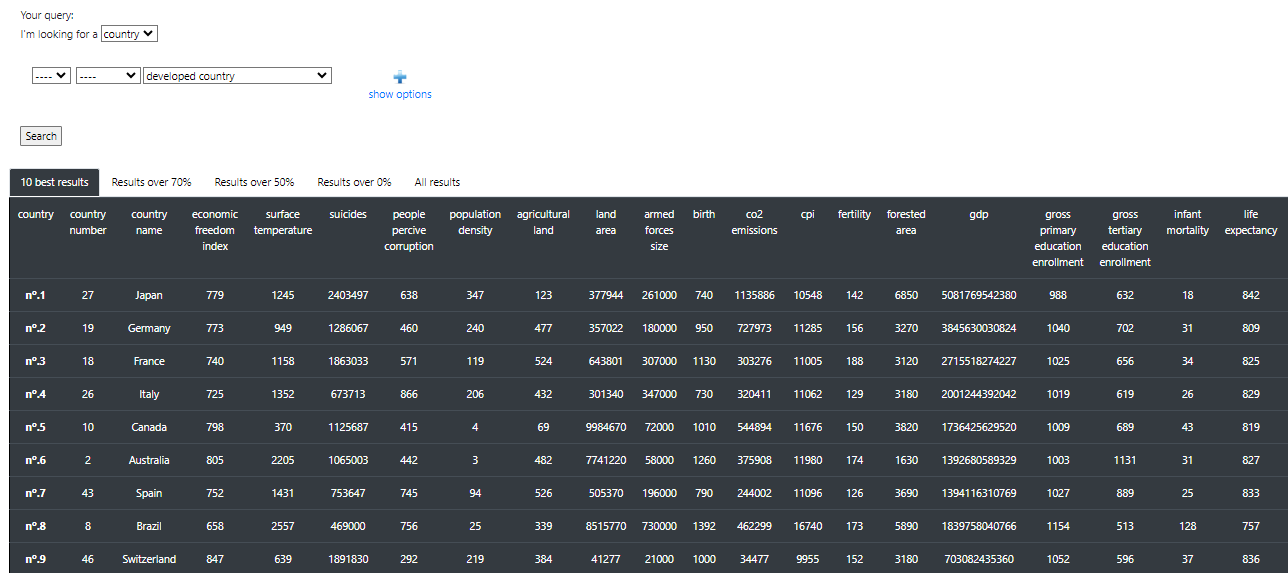
\includegraphics[width=\linewidth]{Images/developed_country.png}
\end{figure}
\begin{figure}
    \centering
    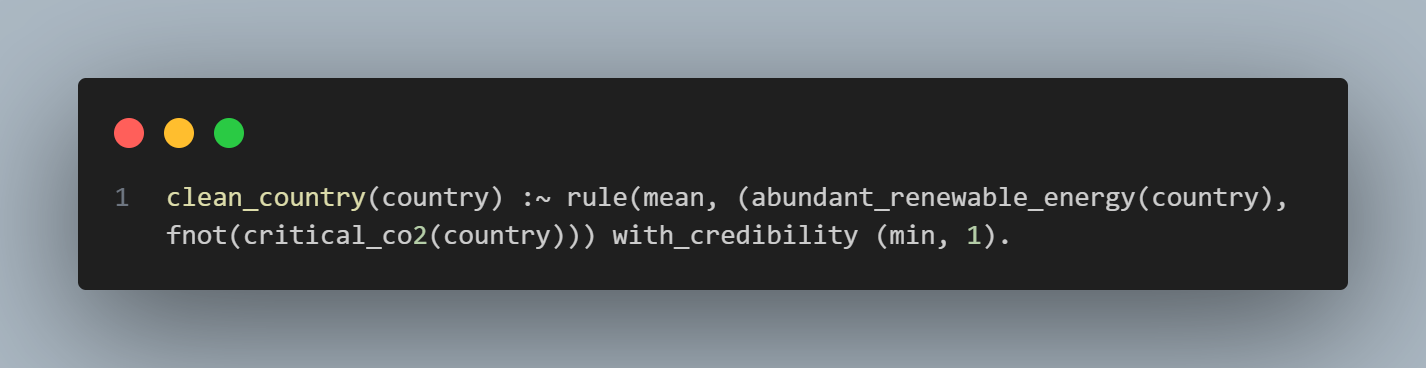
\includegraphics[width=\linewidth]{Images/clean_country.png}
\end{figure}
\end{frame}

\begin{frame}
\frametitle{Consultas}
\slideauthor{Javier Comyn}
\begin{figure}
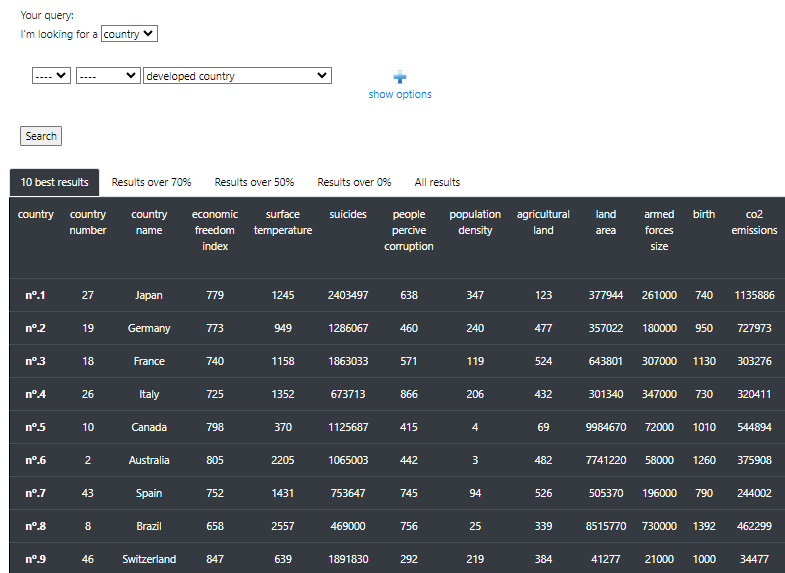
\includegraphics[width=\textwidth]{Images/developed_country (1).png} 
\end{figure}
\end{frame}

\begin{frame}
\frametitle{Consultas}
\slideauthor{Javier Comyn}
\begin{figure}
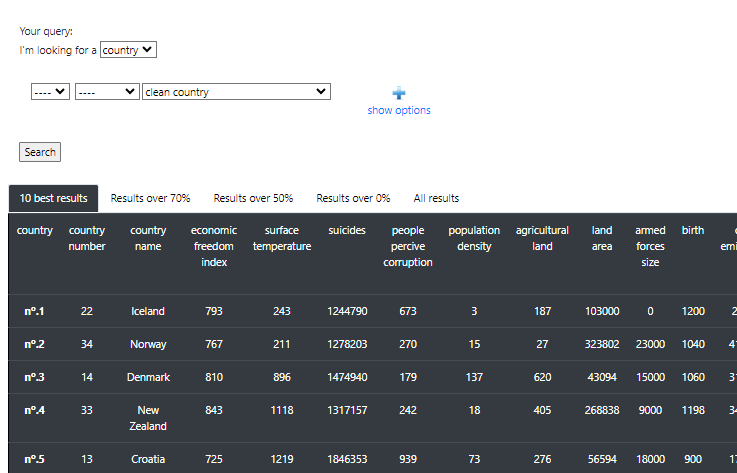
\includegraphics[width=\textwidth]{Images/clean_countries.png} 
\end{figure}
\end{frame}

\begin{frame}
\frametitle{Consultas}
\slideauthor{Javier Comyn}
\begin{figure}
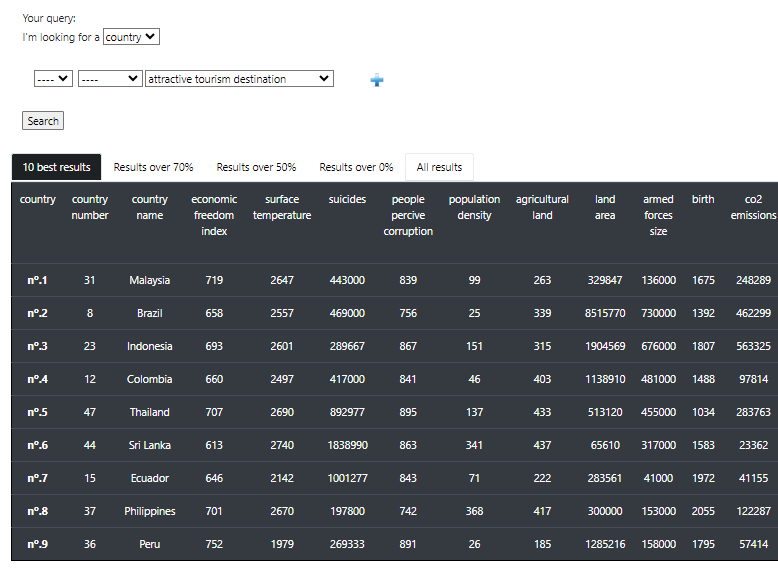
\includegraphics[width=\textwidth]{Images/tourism destinations.png} 
\end{figure}
\end{frame}

\begin{frame}
\frametitle{Resultados Notables}
\slideauthor{Javier Comyn}
    \begin{itemize}
    \item \textbf{Clean Country}: Resultados lógicos :Islandia, Noruega, Dinamarca... Fue inesperado ver a Japón en los puestos más bajos, descubrimos que era por el CO2.
    \item \textbf{Developed Country}: España por encima de economías mejores, demostrando que no sólo eso define el desarrollo de un país.
    \item \textbf{Environmentally Friendly Country}: Se destacaron países con grandes áreas forestales y agrícolas, como Brasil, Canadá y Colombia. 
    \item \textbf{Economically Stable Country}: Tailandia en primera posición, por su bajísmo desempleo. Comprendemos la importancia de la interpretación humana de los resultados.
\end{itemize}
Comparado con modelos tradicionales, la lógica difusa permite hacer interpretaciones más matizadas y completas de la realidad.
\end{frame}

\section{Optimización del modelo}

\begin{frame}{Cálculo de Credibilidad}
\slideauthor{Francisco J. González}
    \begin{block}{Introducción}
        En esta sección se explica cómo se determinaron y automatizaron los cálculos de credibilidad para funciones difusas.
    \end{block}
    \begin{itemize}
        \item Algoritmos en Python para normalizar datos.
        \item Comparación de conjuntos de datos normalizados utilizando MAE (Error Absoluto Medio).
        \item Automatización de consultas en Ciao Prolog
    \end{itemize}
\end{frame}

\begin{frame}{Transformación de Datos}
\slideauthor{Francisco J. González}
    \begin{block}{Problemas}
        \begin{itemize}
            \item Necesidad de tener datos reales en el formato correcto para el algoritmo de normalización.
            \item Obtener y procesar resultados de las consultas.
        \end{itemize}
    \end{block}
    \begin{block}{Soluciones}
        \begin{itemize}
            \item Aplicación de transformaciones a archivos CSV usando Pandas.
            \item Implementación de un programa en C que ejecuta el intérprete Ciao.
        \end{itemize}
    \end{block}
\end{frame}

\begin{frame}{Implementación en C}
\slideauthor{Francisco J. González}
    \begin{block}{Objetivo}
        Crear un programa en C que ejecute el intérprete de Ciao Prolog, automatizando las consultas para las funciones difusas.
    \end{block}
    \begin{itemize}
        \item Ejecución del intérprete Ciao Prolog desde un programa en C.
        \item Envío de consultas a través de la entrada estándar.
        \item Recopilación y procesamiento de resultados a través de la salida estándar.
    \end{itemize}
    \begin{block}{Resultado}
        Automatización completa de las consultas y recolección de datos para el análisis de credibilidad.
    \end{block}
\end{frame}

\begin{frame}{Automatización y Recolección de Datos}
\slideauthor{Francisco J. González}
    \begin{block}{Objetivo}
        Automatizar todo el proceso de consultas y cálculo de credibilidades.
    \end{block}
    \begin{itemize}
        \item Recolección de datos normalizados y valores de verdad para funciones difusas.
        \item Script en Python para consolidar resultados en un archivo de texto.
    \end{itemize}
    \begin{block}{Resultado}
        Comparación de valores de verdad con valores reales para obtener valores de credibilidad de forma automática.
    \end{block}
\end{frame}

\section{Conclusión y Resultados}

\begin{frame}{Desafíos y Soluciones}
\slideauthor{Francisco J. González}
    \begin{block}{Desafíos}
        \begin{itemize}
            \item Recopilación y precisión de datos de múltiples fuentes.
            \item Definición de funciones y reglas apropiadas.
            \item Integración del sistema de lógica difusa con la base de datos.
        \end{itemize}
    \end{block}
    \begin{block}{Soluciones}
        \begin{itemize}
            \item Referencia cruzada de fuentes.
            \item Refinamiento iterativo.
            \item Uso de herramientas robustas y discusiones en equipo.
        \end{itemize}
    \end{block}
\end{frame}

\begin{frame}{Conclusiones}
\slideauthor{Francisco J. González}
    \begin{block}{Éxitos}
        \begin{itemize}
            \item Desarrollo y validación de un modelo socioeconómico basado en lógica difusa.
            \item Precisión considerable en las predicciones dadas por los indicadores.
        \end{itemize}
    \end{block}
    \begin{block}{Limitaciones}
        \begin{itemize}
            \item Dependencia de datos de alta calidad.
            \item Definición de reglas difusas universalmente aplicables.
        \end{itemize}
    \end{block}
\end{frame}

\begin{frame}{Trabajo Futuro}
\slideauthor{Francisco J. González}
    \begin{block}{Mejoras Propuestas}
        \begin{itemize}
            \item Expandir el modelo para incluir más indicadores diversos.
            \item Aplicar el modelo en diferentes regiones y culturas.
            \item Integrar técnicas de aprendizaje automático con lógica difusa.
        \end{itemize}
    \end{block}
    \begin{block}{Potencial}
        \begin{itemize}
            \item Extrapolar la automatización de cálculos de credibilidad para diseñar métodos más precisos en el modelado de funciones difusas.
        \end{itemize}
    \end{block}
\end{frame}

\end{document}
